\documentclass[english,notitlepage,reprint,nofootinbib,twocolumn]{article}  
\usepackage[utf8]{inputenc}
\usepackage{physics,amssymb}
\include{amsmath}
\usepackage{graphicx}         
\usepackage{xcolor}         
\usepackage{hyperref}       
\usepackage{listings}        
\usepackage{subfigure}       
\usepackage{algorithm}
\usepackage[noend]{algpseudocode}
\usepackage{subfigure}
\usepackage{tikz}
\usepackage{multicol}
\usepackage{abstract}
\usepackage{titlesec}

\usetikzlibrary{quantikz}
\hypersetup{
    colorlinks,
    linkcolor={red!50!black},
    citecolor={blue!50!black},
    urlcolor={blue!80!black}}

 \titleformat{\subsection}
  {\normalfont\fontsize{12}{15}\mdseries}{\thesubsection}{1em}{}
 \titleformat{\subsubsection}
  {\normalfont\fontsize{12}{15}\mdseries}{\thesubsubsection}{1em}{}

  
\begin{document}
\title{Project 3 FYS3150} 
\author{Tiril Sørum} 
\date{\today}                             
\maketitle                     

\begin{abstract}
    \textit{This report presents a simulation model for the behavior of particles in a penning trap, specifically focusing on the motion of calcium ions $Ca^+$. It offers insights into particle dynamics and the impact of time-dependent electric field potentials, providing an understanding of the environment within the trap, and its behaviour. All code written for this project, can be viewed in this \href{https://github.com/tirilsg/FYS3150-Project3}{GitHub repository}, at the following link:
  \url{https://github.com/tirilsg/FYS3150-Project3}}
\end{abstract}

\section{Introduction}\label{sec:introduction}

In this report, we present theory needed to simulate the environment within our penning trap, and by implementing these by coding in c++ we manage to create a working model of our system, containing the necessary boundaries. By making use of ODE-solvers such as forward-euler and runge-kutta, we estimate the trajectories of particles within the trap. To study how $Ca^+$ particles in fact will get affected by the system, we use our model to simulate the movement of both a system containing two particles with and without particle interactions, the special case of a single particle, as well as the case of 100 particles with randomly generated initial conditions. For the instance of 100 particles, we also study how particles escape the system during a larger interval of time, when the model for movement both is and is not time-dependant. \\

To make an assessment as to how realistic our model is, we compare the results of our simulations with an analytical solution that we deduce in our report. The accuracy of the ODE-solver trajectories is also assessed by comparing the forward-euler method to the runge-kutta. \\

The report further contains a section in which we both present the results of all our simulations, and discuss what they tell us about the accuracy of the model. Further discussion is provided around the physics behind the model, and why certain changes of conditions yield in certain behaviour of particles within our system. Finally, we draw a conclusion as to the degree of realism of our model. 




\section{Methods}\label{sec:methods}
\subsection{Modelling the environment within the penning trap}
To be able to model our system, we need to take a look at and deduct a couple relevant 
formulas. To begin, we describe the force F on a particle q in an electric field E and
magnetic field B with the formula
\begin{equation}
    F = qE + q(v \times B)
\end{equation}
where v is the velocity of the particle. We can use this in combination with Newtons' second law 
to describe the motion of the particle q in the system. Newtons' second law is expressed 
\begin{equation}
    \sum_{i}{F_i} = ma = m \frac{d^2r}{dt^2}
\end{equation}
where we rewrite a to be expressed as a double derivation. By using these formulas (1) and (2) together, we can obtain expressions for the movement in each of our dimensions x, y and z. The movement is as we can read from the formula (2) independent in each dimension, so we can feel content by deducting our expression for a single dimension; 
\begin{equation}
    \begin{split}
        & qE_x + \left(qv \times B \right)= m \frac{d^2x}{dt^2}  \\
        & \frac{qE_x}{m}+\frac{\left(qv \times B \right)}{m} = \frac{d^2x}{dt^2}    \\
        & \implies  \frac{qE_x}{m}+\frac{q}{m}\left(v_yB_z-v_zB_y \right) = \frac{d^2x}{dt^2} \\
    \end{split}
\end{equation}
By the same logic we get the expression containing movement variables in the y- and z-dimentions;
\begin{equation}
    \frac{qE_y}{m}+\frac{q}{m}\left(v_zB_x-v_xB_z \right) = \frac{d^2y}{dt^2}
\end{equation}
\begin{equation}
    \frac{qE_z}{m}+\frac{q}{m}\left(v_xB_y-v_yB_x \right) = \frac{d^2z}{dt^2}
\end{equation}
In the case of our Penning trap, the magnetic field B only has components in positive z-direction, which we call $B_0$. We use this to simplify our expressions further. Additionally, we use the definition of electric potential; 
$$E=- \Delta V$$
where the potential V is expressed 
\begin{equation}
    V(x,y,z)=\frac{V_0}{2d^2}\left(2z^2-x^2-y^2\right)
\end{equation}
where d is $\sqrt{z_0^2+r_0^2/2}$, and $V_0$ is the potential applied to the particles, and thereby express the strength of our electric field in each dimension; \\
\begin{equation}
    E_x=\frac{V_0x}{d^2}   ,   E_y=\frac{V_0y}{d^2}   ,   E_z=\frac{2V_0z}{d^2} 
\end{equation}
If we wish to express the potential V as time-dependent, we will have to replace the value $V_0$ in this expression with 
\begin{equation}
    V_0(1+f\cos{(w_Vt)})
\end{equation}
where f is a constant amplitude.

If a system contains multiple particles, their movement will be affected by each-other, with a force described by coulomb's law:
\begin{equation}
    F=k_e \frac{q_1q_2}{r^2}
\end{equation}
The model for this system does trap the particles inside in the z-direction, but an escape from the system is possible in both x- and y-directions. 

 

\subsection{Analytic estimation of movement of particles within our system}

If we so wish, these expressions (3), (4) and (5) can be restructured in a way to resemble the 
equations of motion;
\begin{equation}
    \begin{split}
        & \frac{d^2x}{dt^2} - \frac{qE_x}{m} -  \frac{q}{m}\left(\frac{dy}{dt}B_0 \right) = 0 \\
        & \implies \frac{d^2x}{dt^2} - \frac{1}{2} \frac{q}{m} \frac{V_0}{d^2}2x -  \frac{q}{m}\left(\frac{dy}{dt}B_0 \right) = 0\\                      
        & \ddot{x} - \frac{1}{2} w_z^2x -  \dot{y}w_0 = 0 \\
    \end{split}
\end{equation}
---------------------------------------------------------------
\begin{equation}
    \begin{split}
        &\frac{d^2y}{dt^2} -\frac{qE_y}{m}+\frac{q}{m}\left(\frac{dx}{dt}B_0 \right) = 0 \\
        & \implies \frac{d^2y}{dt^2} -\frac{1}{2}\frac{q}{m}\frac{V_0}{d^2}2y + \frac{q}{m}\left(\frac{dx}{dt}B_0 \right) = 0\\
        & \ddot{y} -\frac{1}{2} w_z^2y + \dot{x}w_0  = 0\\
    \end{split}
\end{equation}
---------------------------------------------------------------
\begin{equation}
    \begin{split}
        & \frac{d^2z}{dt^2} - \frac{qE_z}{m} = 0 \implies \frac{d^2z}{dt^2} -\frac{1}{2}\frac{q}{m}\frac{V_0}{d^2}4z = 0  \\
        & \ddot{z} -w_z^2 z = 0 \\
    \end{split}
\end{equation}
when we set $w_0= \frac{qB_0}{m}$  and $w_z=\frac{2qV_0}{md^2}$, and use the notation $\dot{u}$ and $\ddot{u}$ for the derivative and double-derivative. \\

We're interested in the position of the particle q, which means we have to find the general solution for each of these expressions (10), (11) and (12). We know that the equation (12) has the general solution computed by integration: 
\begin{equation}
    %z(t)=\int{(\int{w_z^2dt})dt+C_1t+C_2} \\
    z(t)=z_0\cos{w_zt} + \frac{v_{z0}}{w_z}sin(w_zt) \\
\end{equation}

%where $C_1$ and $C_2$ are constants that can be decided if we know the initial condition of our system. \\%

To be able to describe the position of the charge q in the x and y-dimensions, we have to make use of a trick - we rewrite the equations (10) and (11) by introducing the function $f(t)=x(t)+iy(t)$, that we can use rewrite to a single differential equation by: 
$$f(t)=x(t)+iy(t)$$
\begin{equation}
    \dot{f}=\frac{df}{dt}=\frac{dx}{dt}-i\frac{dy}{dt} \\
\end{equation}
\begin{equation}
    \ddot{f}=\frac{d^2f}{dt^2}=\frac{d^2x}{dt^2}+i\frac{d^2y}{dt^2} \\
\end{equation}
We can rewrite the expressions (10) and (11) to compliment (14) and (15): 
$$\ddot{y} -\frac{1}{2} w_z^2y + \dot{x}w_0  = 0 = i\frac{d^2y}{dt^2}-\frac{1}{2} w_z^2y + \frac{dx}{dt}w_0  $$
$$\ddot{x} - \frac{1}{2} w_z^2x -  \dot{y}w_0 = 0 = \frac{d^2x}{dt^2}-\frac{1}{2} w_z^2x  - i\frac{dy}{dt}w_0  $$
We know since both expressions are equal to 0, the sum of them both will also be 0. Therefore, we can:  
$$\frac{d^2x}{dt^2}-\frac{1}{2} w_z^2x  - i\frac{dy}{dt}w_0 + i\frac{d^2y}{dt^2}-\frac{1}{2} w_z^2y + \frac{dx}{dt}w_0 = 0 $$

$$\frac{d^2x}{dt^2}+ i\frac{d^2y}{dt^2} +(\frac{dx}{dt}w_0- i\frac{dy}{dt}w_0) -(\frac{1}{2} w_z^2y +\frac{1}{2} w_z^2x) = 0 $$
We can insert the expressions for (13) and (14) into this equation, and we get the expression: 
$$\ddot{f} +w_0\dot{f} -(\frac{1}{2}w_z^2)(y + x) = \ddot{f} +w_0\dot{f} - \frac{1}{2}w_z^2f=0 $$

We have the solution to this differential equation 
$ f(t)=A_+e^{-i(w_+t+\phi_+)}+A_-e^{-i(w_-t+\phi_-)}$ where $\phi_+ $
and $\phi_-$ are constant phases, the amplitudes $A_+$ and $A_-$ are positive, and 
\begin{equation}
w_{\pm}=\frac{w_0 \pm \sqrt{w_0^2-2w_z^2}}{2}
\end{equation}
The coordinates x(t) and y(t) can be extracted from this expression $f(t)$, by rewriting it to contain sin and cos, instead of real and imaginary numbers; 
\begin{equation}
    \begin{split}
        & x=A_+ \cos{(w_+t+\phi_+)}+ A_-\cos{(w_-t+\phi_-)}\\
        & y=-A_+\sin{(w_+t+\phi_+)}- A_-\sin{(w_-t+\phi_-)} \\
    \end{split}
\end{equation}

We put constraint on our values $w_0$ and $w_z$ so that the amplitude of our equation $f(t)$ remains finite when t approaches infinity. For this to be possible, both our values for $w_0$ and $w_z$ need to be real, which means our discriminant under the square root in equation (16) ${w_0^2-2w_z^2}=( \frac{qB_0}{m})^2-2(\frac{2qV_0}{md^2})^2 \geq 0$. We can rewrite this constraint; $B_0^2 d^4-8V_0^2 \geq 0$. \\

Furthermore, we know that when $A_+$ and $A_-$ have the same phase (when they have the same sign), they interfere in such a way that the function $f(t)$ will achieve it's maximum possible amplitude. This expression describes, practically, the upper bounds for the particle q's distance from the origin in the xy-plane. On the other hand, we can describe the particles lower bounds when $A_+$ and $A_-$ are in opposite phases and the interference work destructively:\\
$$f_+(t)=A_+e^{-i(w_+t+\phi_+)}+A_-e^{-i(w_-t+\phi_-)}$$
$$f_-(t)=A_+e^{-i(w_+t+\phi_+)}-A_-e^{-i(w_-t+\phi_-)}$$ 
Since we're interested in the bounds in the xy-plane, we only look at the elements which exist in these dimensions, and to make sure that they're in the correct phases, we only need to express: 
$R_+=\abs{(A_+ + A_-)}$ and $R_-=\abs{(A_+ - A_-)}$ \\


\subsection{A special case}
In the special case that we're dealing with a single particle within our Penning trap at a time, with\\ $x(0)=x_0$, $y(0)=0$, $z(0)=z_0$\\
$\dot{x}(0)=0$, $\dot{y}(0)=\dot{y}_0$, $\dot{z}(0)=0$\\ the position of the particle will be described by $\phi_- = \phi_+ = 0$ and $A_+=\frac{v_0+w_-x_0}{w_--w_+}$, $A_-=-\frac{v_0+w_+x_0}{w_--w_+}$. 
We can take advantage of this to model how a single particle will be affected by the system, and consequently learn more about the forces at work.  \\

We can now, if we wish, create a model for a particle $q$ within a system Penning trap, with position given by the expressions deduced up-until now.

\subsection{Numeric estimation of movement of particles within our system}
We can simulate one, or multiple particle's movement within the trap by expressing the forces from the electric and magnetic fields, as well as the forces between the particles (if the trap contains multiple particles). A simulation can be ran by expressing these forces, and thereafter evolve the system in time, a tiny step at a time, by either forward-Euler-method or Runge-Kutta-method. \\
\subsubsection{The Runge-Kutta method}
The Runge-Kutta method approximates the solution to an ODE, and is defined: 
\begin{align*}
k_1 &= h \cdot f(t_n, y_n) \\
k_2 &= h \cdot (t_n + \frac{h}{2}, y_n + \frac{k_1}{2}) \\
k_3 &= h \cdot (t_n + \frac{h}{2}, y_n + \frac{k_2}{2}) \\
k_4 &= h \cdot f(t_n + h, y_n + k_3) \\
y_{n+1} &= y_n + (k_1 + 2k_2 + 2k_3 + k_4)\frac{1}{6}
\end{align*}
where y is the value we wish to approximate the next value for, and is dependent on time, h is the stepsize, and $f(t, y)$ is the derivative of y with respect to t. When talking about position of a particle, this f will correspond to the particles velocity, and we can use $\dot{r}=v$ and $\dot{v}=F/m$ to estimate these values for each step. \\

\subsubsection{The Forward-Euler method}
The Forward-Euler method for solving ODEs is defined:
\begin{align*}
y_{n+1} &= y_n + h \cdot f(t_n, y_n)
\end{align*}
where the definitions of variables are the same as for the definition of the Runge-Kutta method.\\

From these definitions, one would assume that the estimations done by Runge-Kutta will be more accurate than the ones estimated by Forward-Euler. To both check that this assumption is valid, and that the simulation that utilizes these methods are accurate, we need to perform an analysis of these errors. 


\subsection{Estimation of errors}
The analysis of errors can be done by both comparing the results of simulation by Runge-Kutta by the results of simulation by Forward-Euler, and comparing the movement as results of these simulations to the movement estimated by our equations (13) and (17). In the case of comparison between our ODE-solver, and analytical equation simulations we can simply estimate an absolute error for each step in time our ODE-solver performs: 
\begin{equation}
    %Er=\sqrt{(s_x-a_x)^2+(s_y-a_y)^2+(s_z-a_z)^2} \\
    Abs=\abs{pos_{simulated}-pos_{analytical}} 
\end{equation}
where s symbolizes the simulated estimated value and a symbolizes the analytical estimated value for each coordinate. This operation simply compares our movement by ODE to the value one would expect, given by the analytical formulas. Often times, the size of this absolute error compared to the actual value can be quite interesting. This ratio is called relative error, and can be simply expressed as; 
\begin{equation}
    Rel=\frac{Abs}{pos_{analytical}}
\end{equation}
The rate of convergence for the relative error can furthermore be pretty interesting. We express this term: 
\begin{equation}
    r_{\text{err}} = \frac{1}{3}\sum_{k=2}^4\frac{\log (\Delta_{\text{max},k}/\Delta_{\text{max},k-1})}{\log (h_{k}/h_{k-1}) }
\end{equation}
where $\Delta_{\text{max},k} = \max_i |\mathbf{r}_{i, \text{exact}} - \mathbf{r}_{i}|$


\subsection{Numbers}
For the model of our penning trap model, we need to implement a couple numbers and units. We express mass in u, charge in e, and both length and time with a base $\mu m$ and $\mu s$, since our model deals with small values: \\
$k_e = 1.38935333 \times 10^5 \frac{u (\mu m)^3}{(\mu s)^2e^2}$\\
$B_0 =  9.65 \times 10 \frac{u}{(\mu s)e}$ \\
$V_0 = 2.41 \times 10^6 \frac{u (\mu m)^2}{(\mu s)^2e}$ \\
$d = 500\,\mathrm{\mu m}$ \\
We use these forms of units in our model for the penning trap. \\
We simulate $Ca^+$ particles, with mass m = 40.078 u and q = 1 e. 

\subsection{Tools}
We need a couple of tools to help us implement our model. The first of these tools that we make use of is c++ coding, which we use to implement two classes; a class Particle defines a particle by charge, mass, position- and velocity-vectors, and a class PenningTrap that defines the entire environment within the penning trap, and contains functions for movement-estimation by both Runge-Kutta and Forward-Euler. The PenningTrap function we write, also takes into consideration whether we wish to model a system where we take into account interaction between particles, as well as time dependency. 

By using coding in c++, we also implement functions for saving relevant data in .txt and .bin files, to be interpreted and analyzed elsewhere. Another independent function is implemented, which fills a penning trap with a number of particles with randomly generated initial positions and velocities. The c++ code makes great use of "armadillo", which lets us easily perform calculations with vectors. \\

Another tool that is necessary to perform our analysis, is python coding. By making use of the python libraries matplotlib, numpy and pyarma, we import the data files created by c++ code, and visualize the data in forms of plots in both 2D and 3D. By importing this data to python, a simple error-analysis can additionally be performed. 


\section{Results}\label{sec:results}
We implement the program code in c++ described in section 2.7, using the theory presented previously. Thereafter, we define two $Ca^+$ particles by their initial conditions; \\

Particle 1:\\
$(x_0, y_0, z_0) = (20, 0, 20)\mu m $ \\
$(v_{x0}, v_{y0}, v_{z0}) = (0, 25, 0)\mu m / \mu s$\\

Particle 2: \\
$(x_0, y_0, z_0) = (25, 25, 0)\mu m $\\
$(v_{x0}, v_{y0}, v_{z0}) = (0, 40, 5)\mu m / \mu s$ 

\subsection{Particle1 alone in the penning trap}
We simulate the time-independent movement of particle1 inside of the penning trap during a time interval $50 \mu s$, with 4000 steps, and movement estimated by the Runge-Kutta method. The data is stored in a .txt file "particle1motion.txt" and imported into python, where we check the accuracy of our model by comparing the estimated movement in z-direction with the expected (analytic) movement:
\begin{figure}[H]
    \centering
    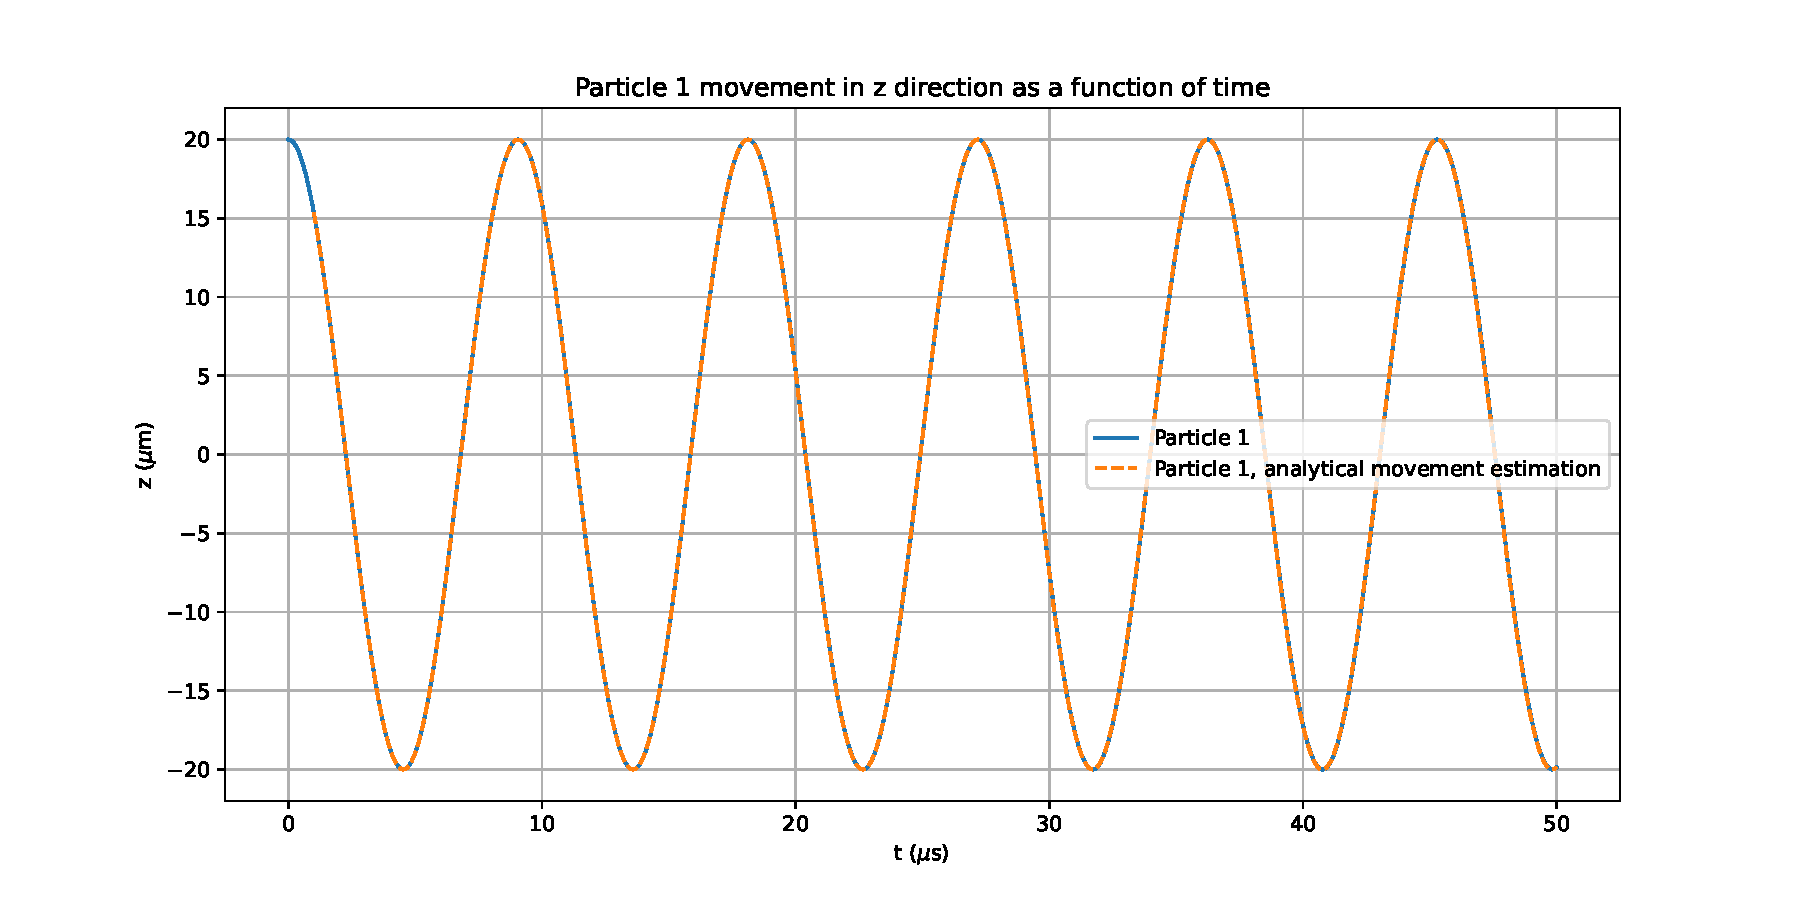
\includegraphics[width = .45\textwidth]{zdir_particle1motion.pdf} 
    \caption{Figure showing the movement of particle 1 in the z-direction, both as simulated by our model in c++, and estimated by our analytic formula. Saved as "zdir\textunderscore particle1motion.pdf".}
    \label{fig: ee251}
\end{figure}

\subsection{Particle1 and particle2 in the penning trap}
We want to test the model by checking how both the particles move when we do not, and when we do take particle interaction into consideration. This is done by performing two different simulations, with different arguments for particle interaction, and no time dependency. The simulations are both ran for a time interval $50 \mu s$, with 4000 steps, and movement estimated by Runge-Kutta. The data is saved in files "withoutinteraction.txt" and "withinteraction.txt", and imported into python, where the data is visualized in a couple different ways. 

\subsubsection{Movement of particle 1 and 2 in the xy-plane}
We create a plot showing the movement of both particles in the xy-plane, with and without particle interaction: 
\begin{figure}[H]
    \centering
    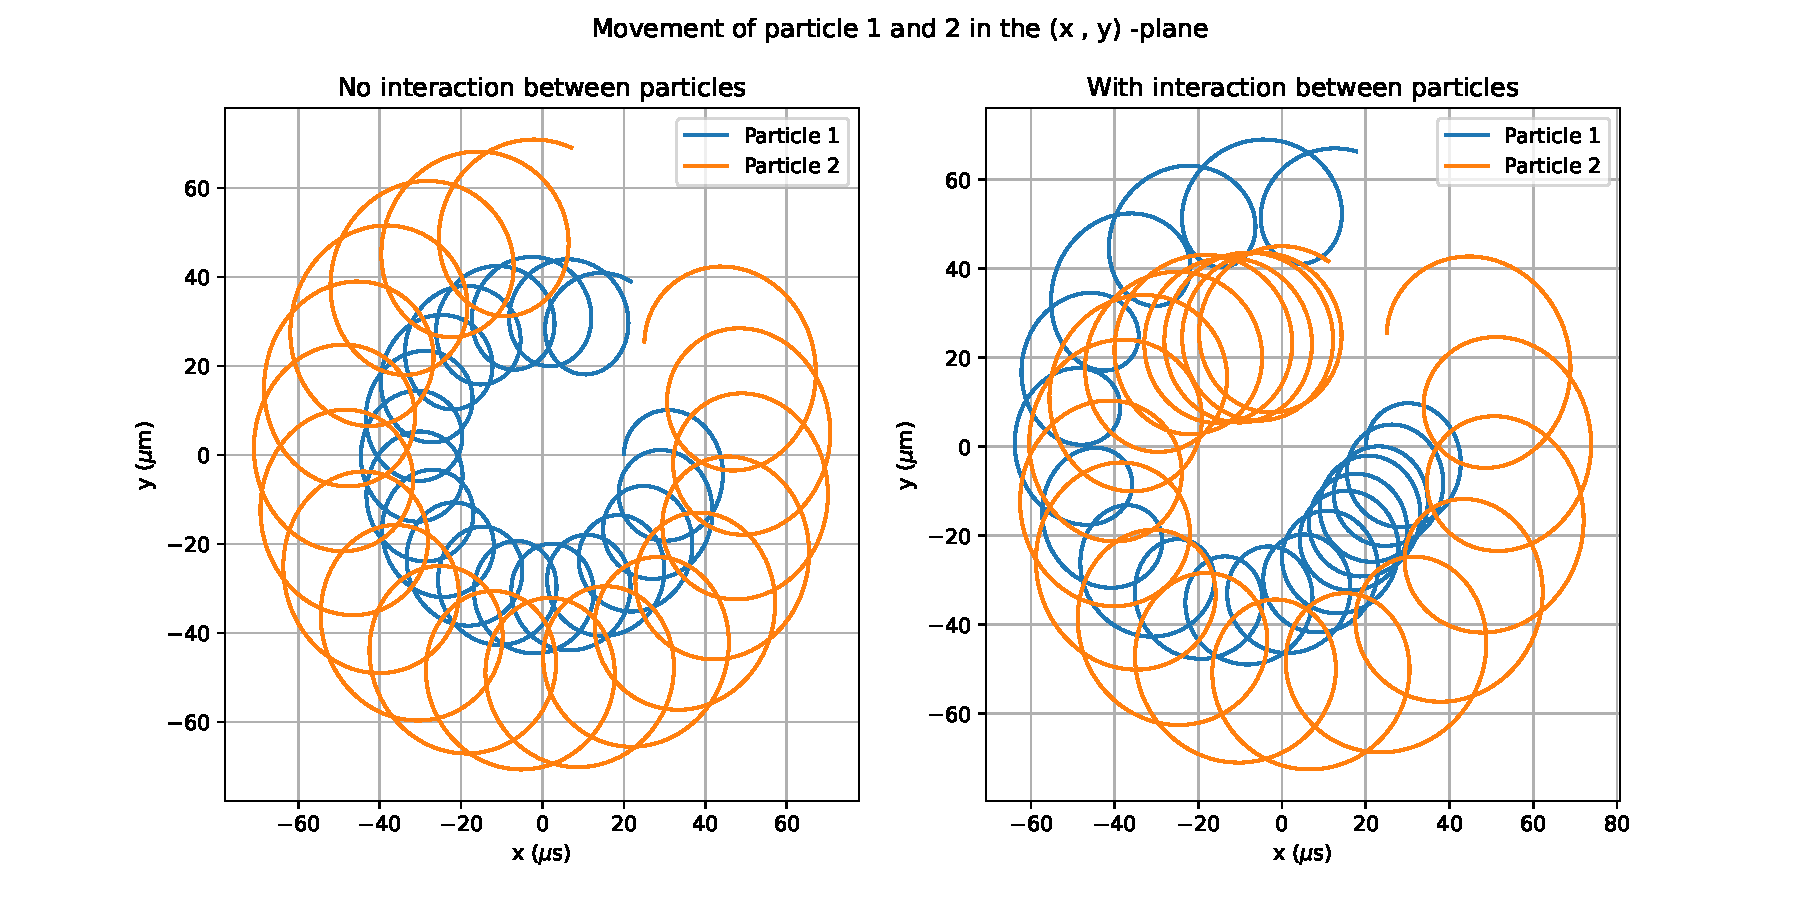
\includegraphics[width = .45\textwidth]{xy_movement.pdf} 
    \caption{Plots visualizing the movement of particle 1 and particle 2 in the xy-plane, with and without a consideration to particle interaction. Saved as "xy\textunderscore movement.pdf".}
    \label{fig: ee251}
\end{figure} 

Subsequently, it could be interesting to see how this movement looks as a further function of time. We make this plot: 
\begin{figure}[H]
    \centering
    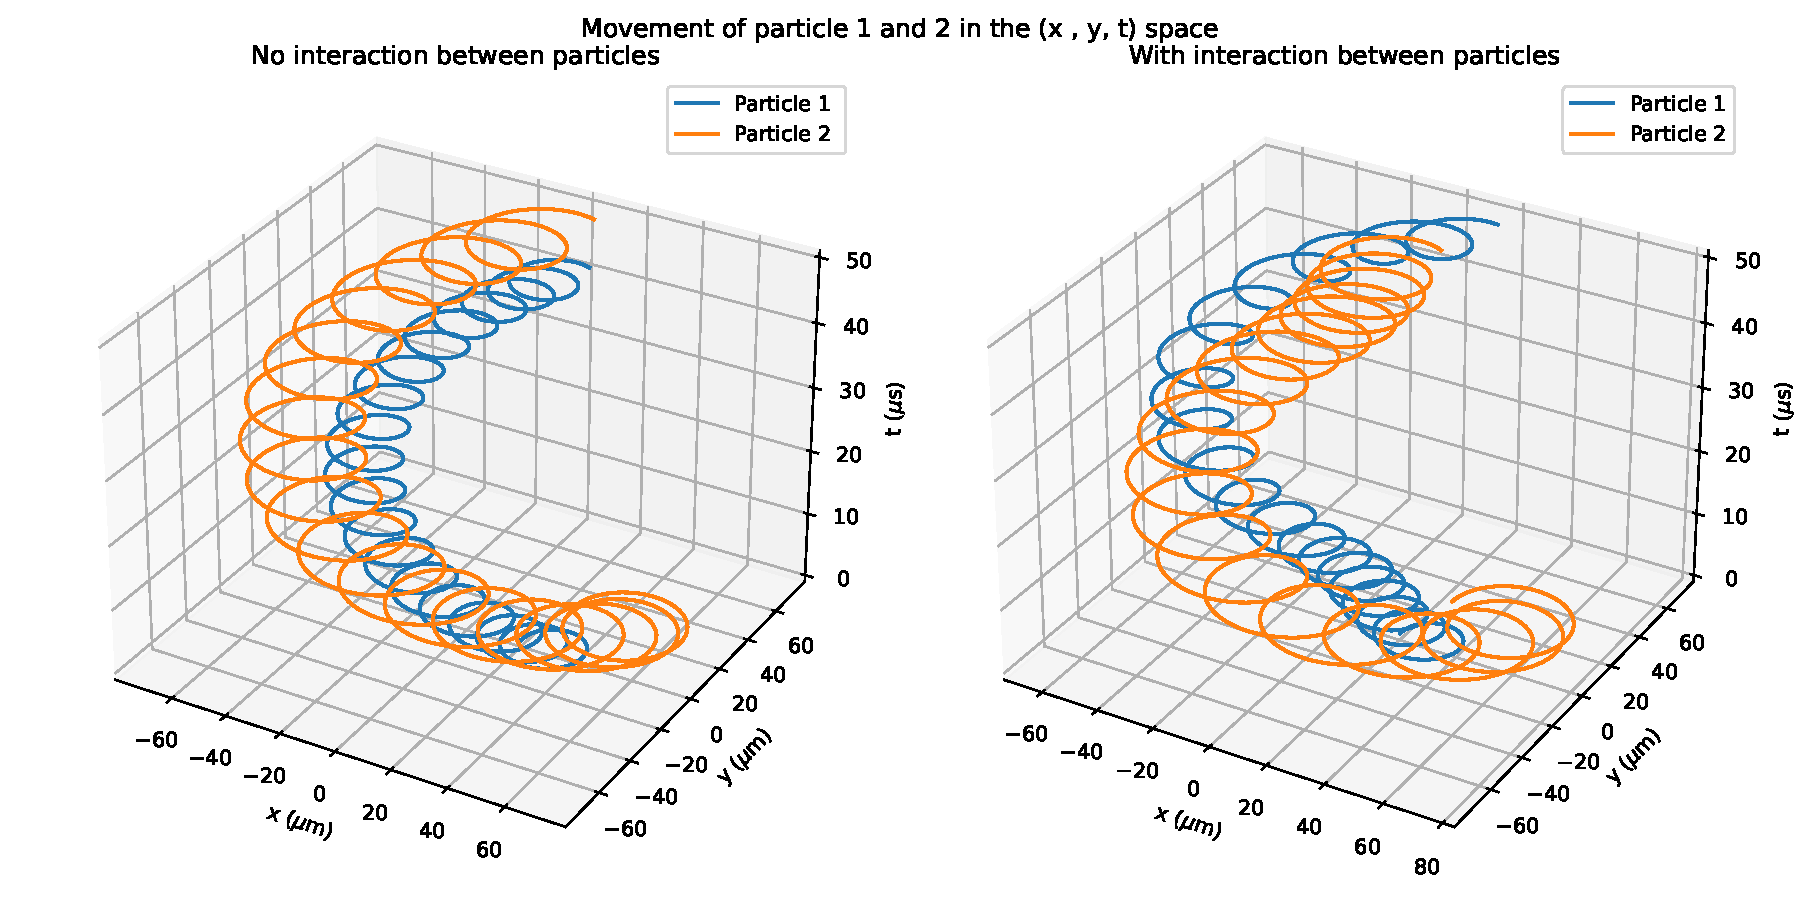
\includegraphics[width = .45\textwidth]{xyt_movement.pdf} 
    \caption{Plots visualising the same data set as Figure 2, as a function of development in time as well. Movement of particles 1 and 2 in the xy-plane as a function of time (x,y,t). Saved as "xyt\textunderscore movement.pdf"}
    \label{fig: ee251}
\end{figure} 

\subsubsection{Phase space plots}
We make plots showing the trajectories (x , $v_x$) with and without interaction.
\begin{figure}[H]
    \centering
    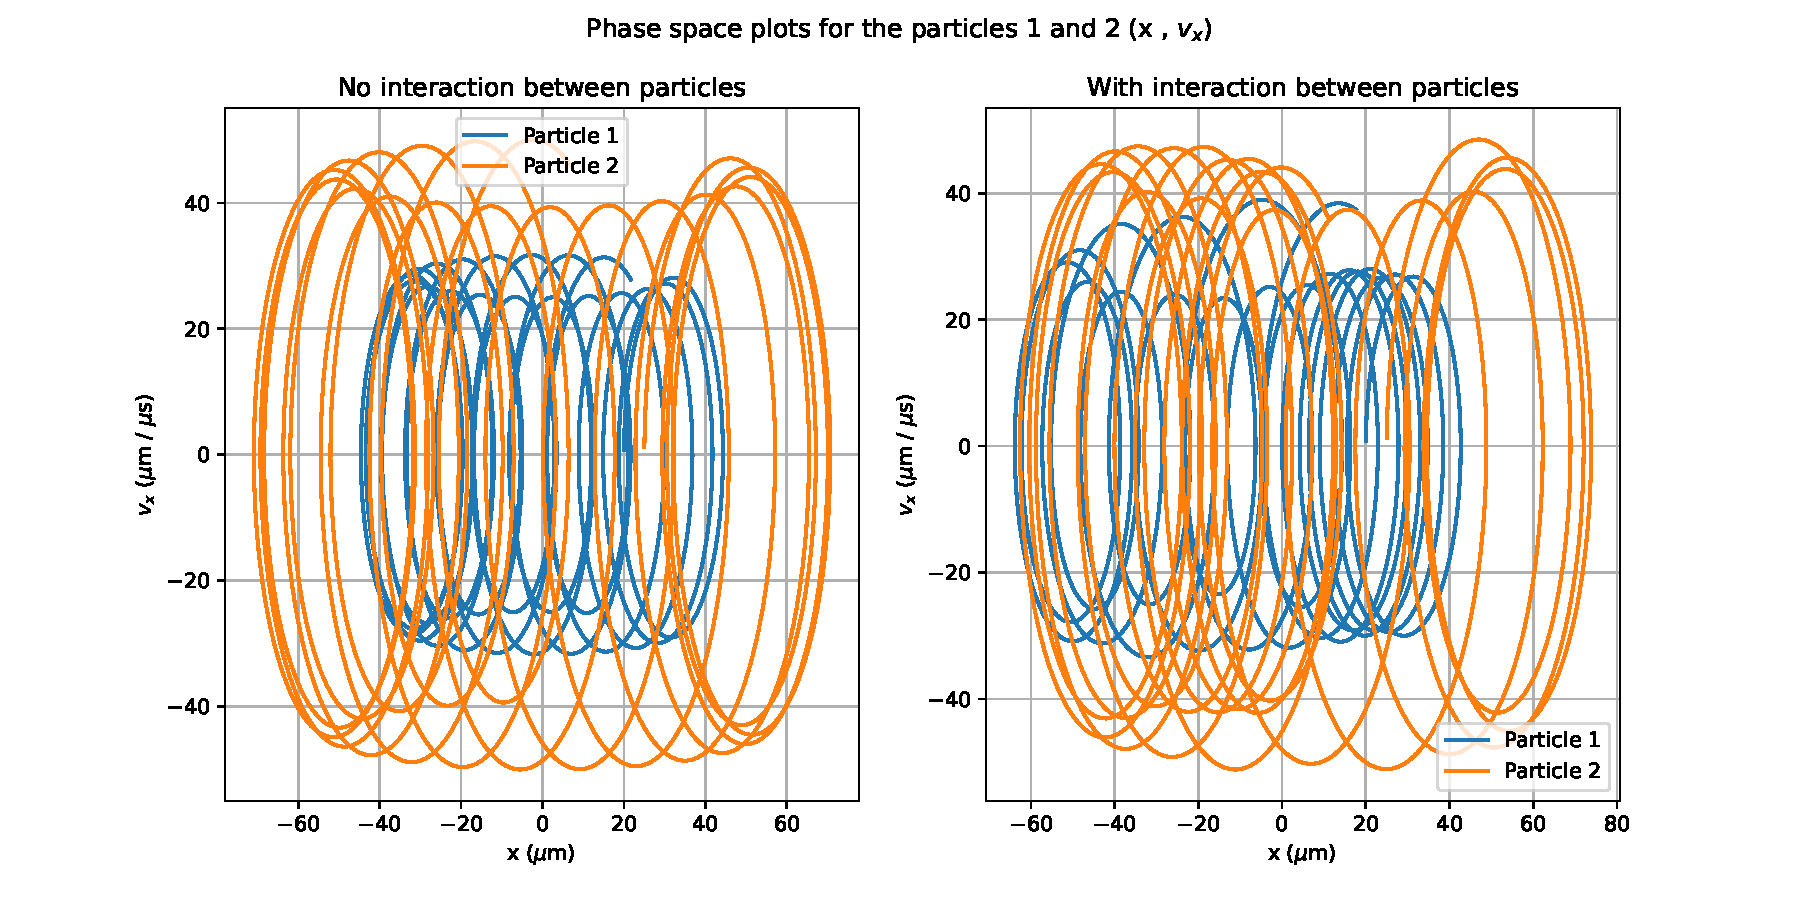
\includegraphics[width = .45\textwidth]{Phasespace_(x,v_x).pdf} 
    \caption{Plots visualizing phase space plots (x , $v_x$) with and without interaction between the particles. Saved as "Phasespace\textunderscore (x,v\textunderscore x).pdf".}
    \label{fig: ee251}
\end{figure} 
%insert "Phasespace_(x,v_x).pdf"
Also in this case, the development as a function of time seems interesting, so we create another plot visualizing the trajectories (x, $v_x$ , t): 
\begin{figure}[H]
    \centering
    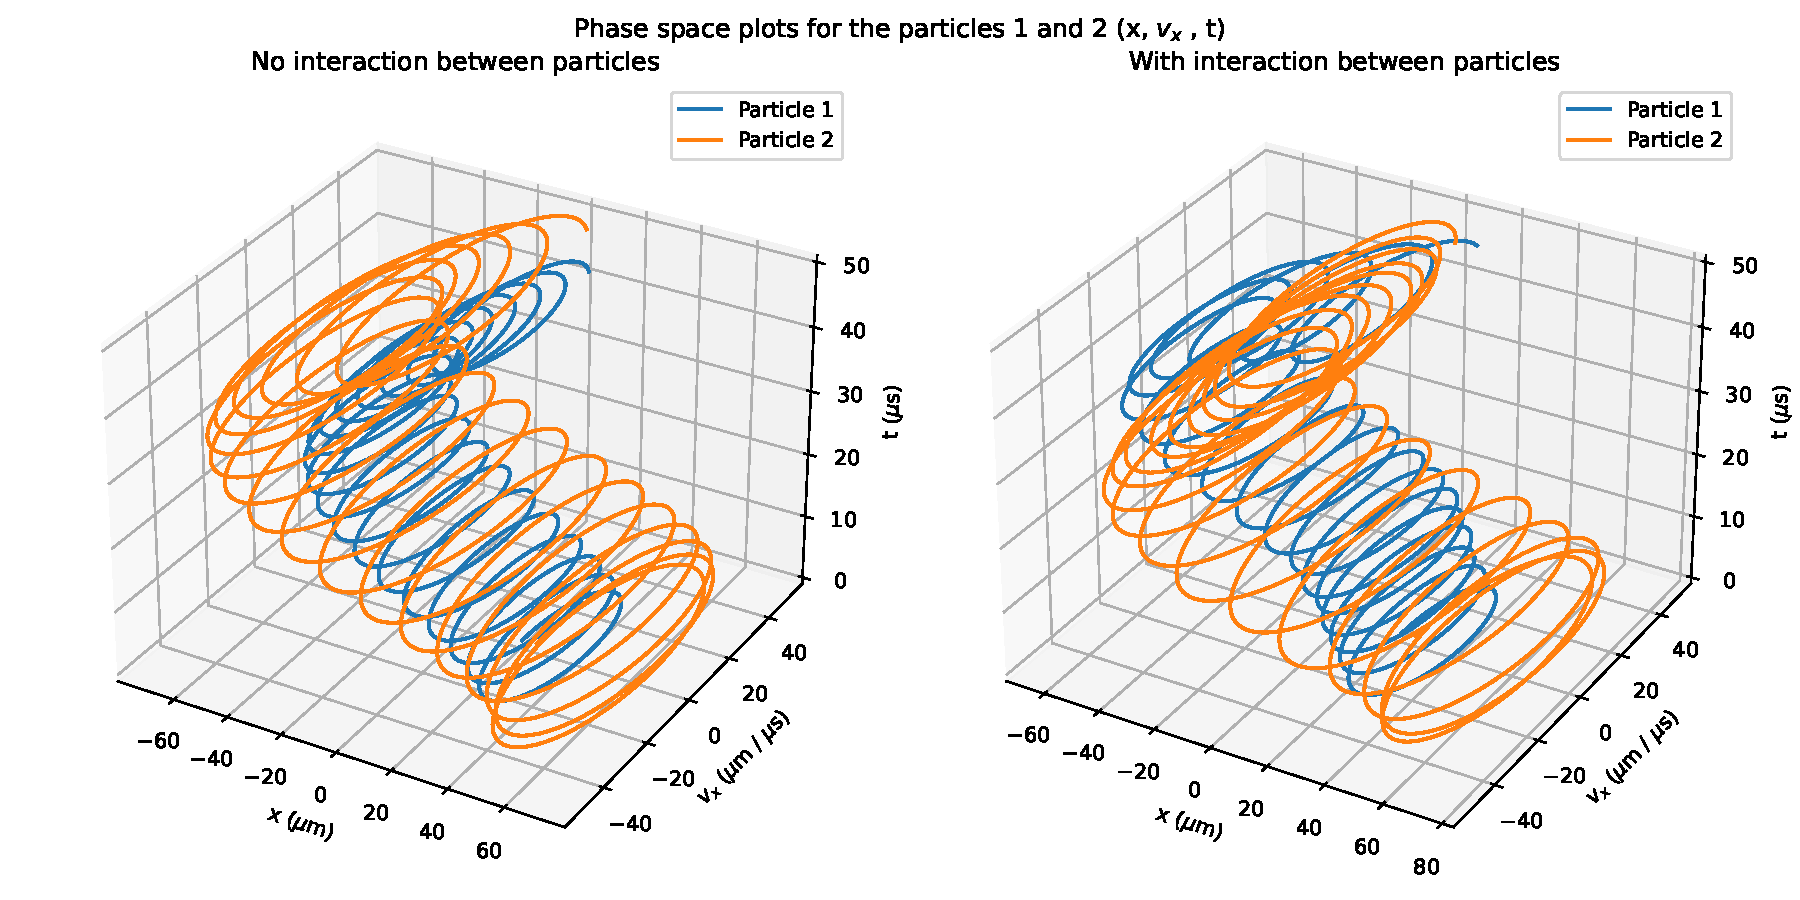
\includegraphics[width = .45\textwidth]{Phasespace_(x,v_x,t).pdf} 
    \caption{Plot showing how the phase space plots in figure 4 develops as time advances. Saved as "Phasespace\textunderscore (x,v\textunderscore x,t).pdf".}
    \label{fig: ee251}
\end{figure} 

The trajectories for the z-dimension is also interesting, so we subsequently make the same plots as previously for this instance: 
\begin{figure}[H]
    \centering
    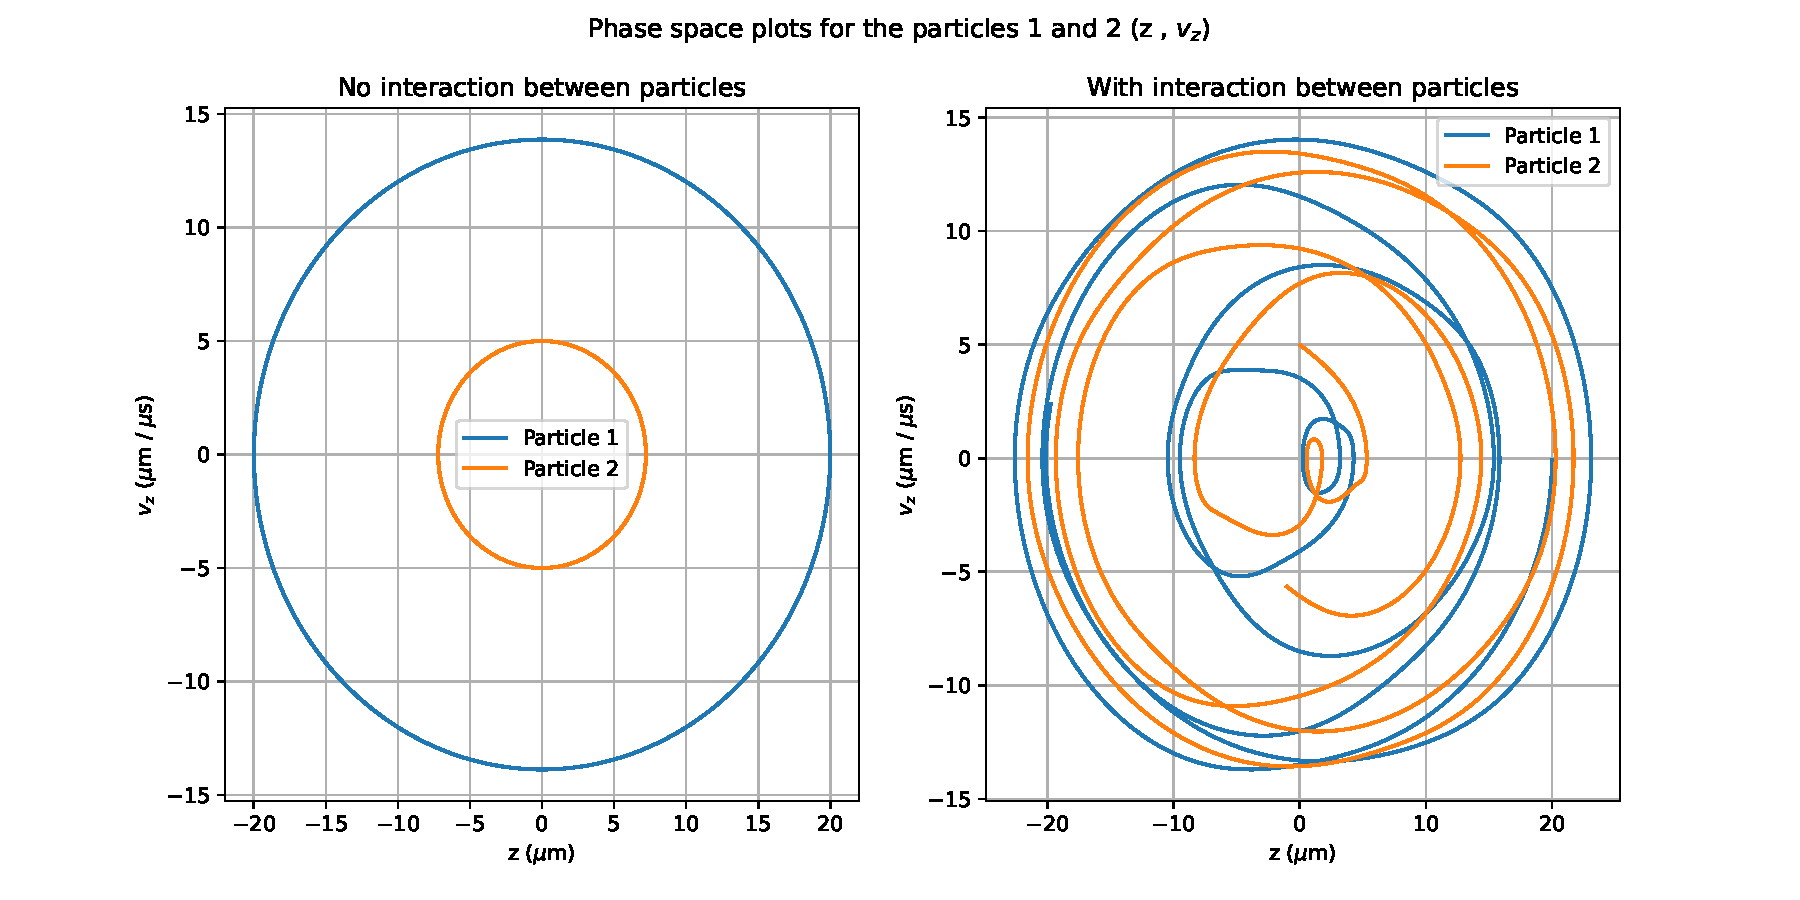
\includegraphics[width = .45\textwidth]{Phasespace_(z,v_z).pdf} 
    \caption{Plots visualizing phase space plots (z , $v_z$) with and without interaction between the particles. Saved as "Phasespace\textunderscore (z,v\textunderscore z).pdf".}
    \label{fig: ee251}
\end{figure} 
\begin{figure}[H]
    \centering
    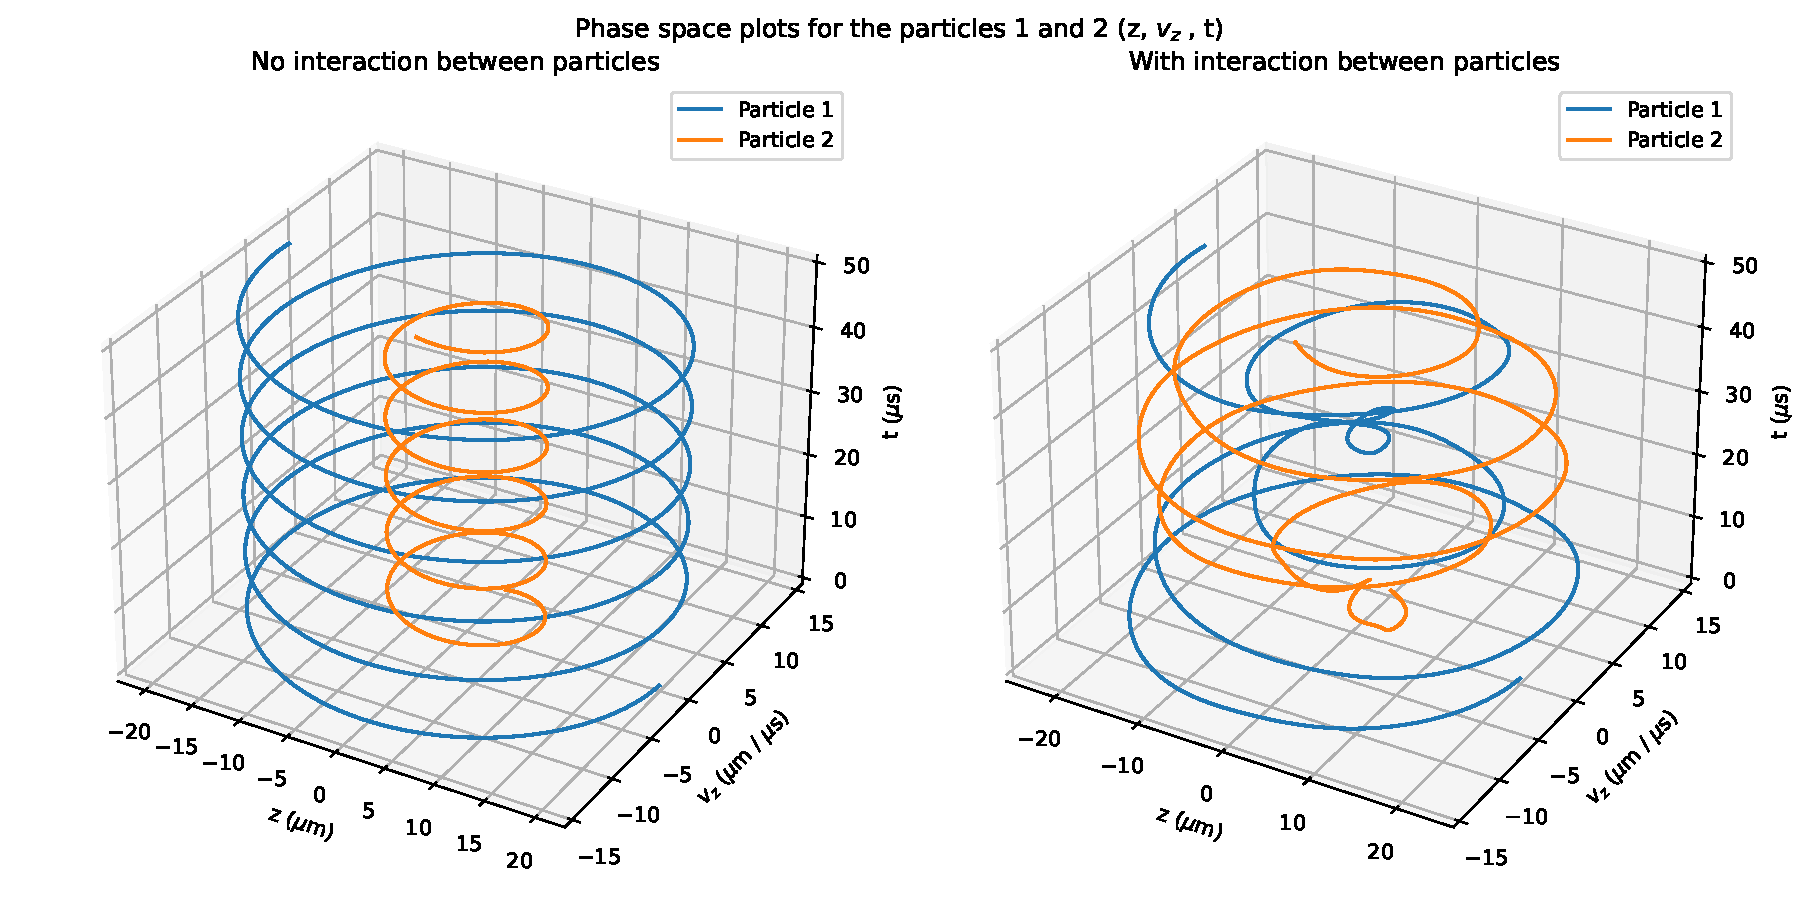
\includegraphics[width = .45\textwidth]{Phasespace_(z,v_z,t).pdf} 
    \caption{Plot showing how the phase space plots in figure 6 develops as time advances. Saved as "Phasespace\textunderscore (z,v\textunderscore z,t).pdf".}
    \label{fig: ee251}
\end{figure} 
\pagebreak
\subsubsection{3D plots for movement in the xyz-space}
Like we did for the movement of the particles in the xy-plane, we now visualize the movement of the particles within the entire xyz-space, both with and without interactions: 
\begin{figure}[H]
    \centering
    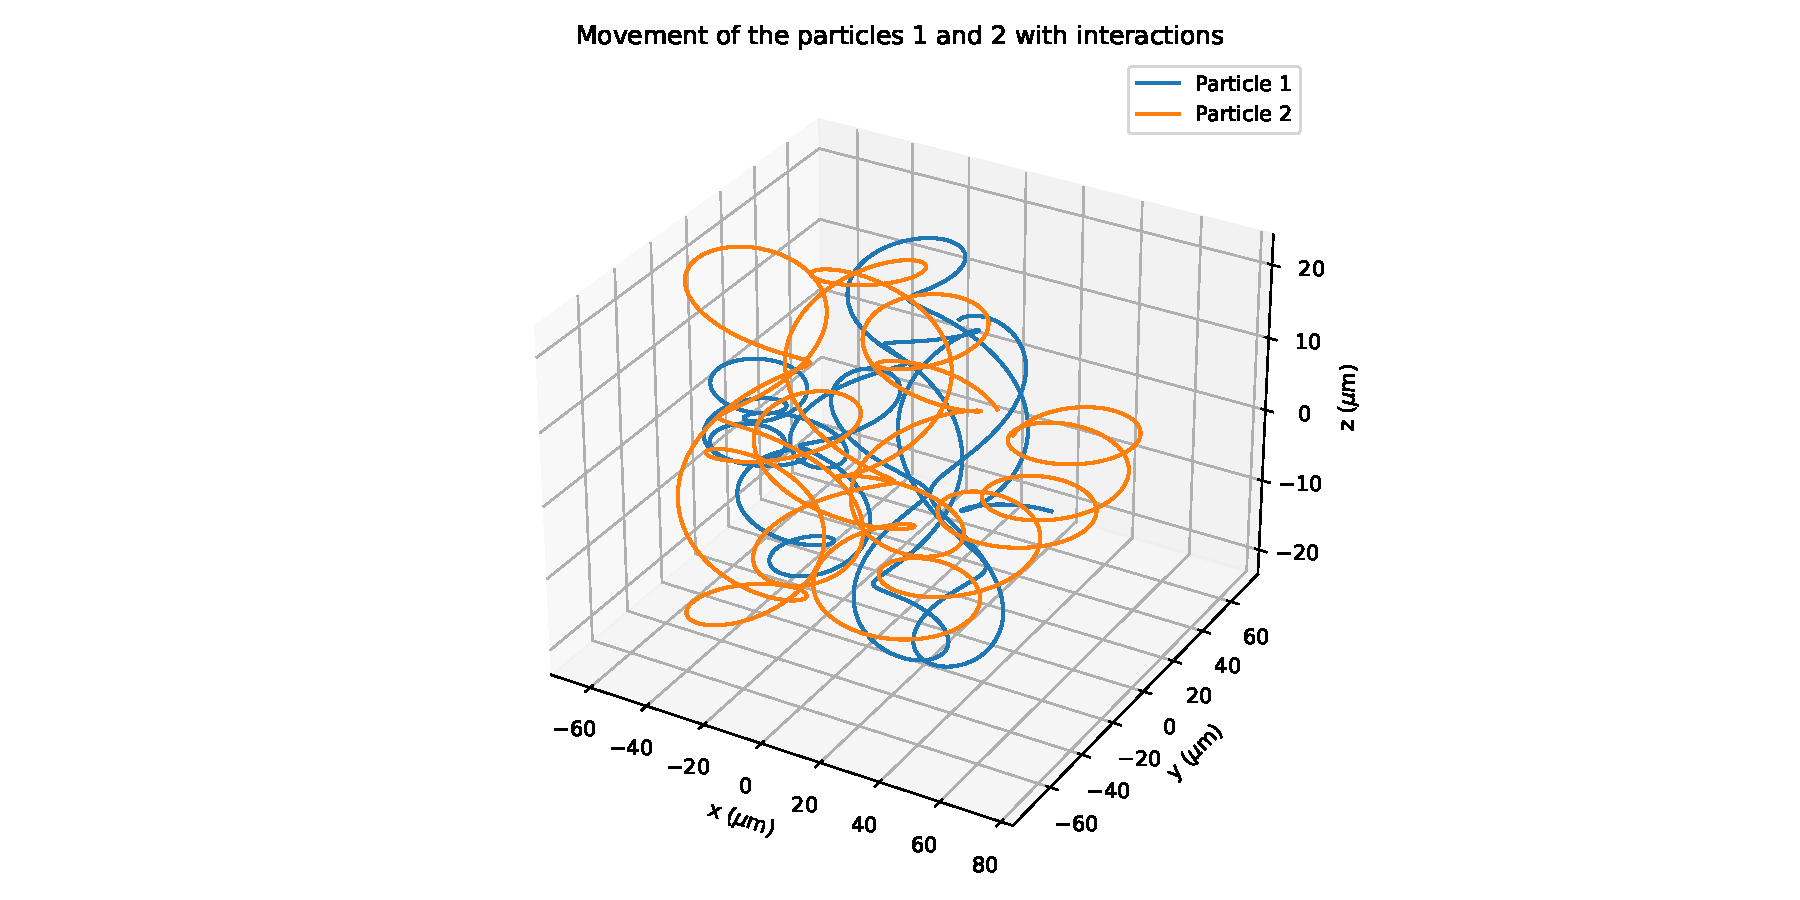
\includegraphics[width = .45\textwidth]{3Dwithinteractions.pdf} 
    \caption{3D plot showing the movement of particle 1 and particle 2 in the xyz-space, when the particles interact with each other. Saved as "3Dwithinteractions.pdf".}
    \label{fig: ee251}
\end{figure} 

\begin{figure}[H]
    \centering
    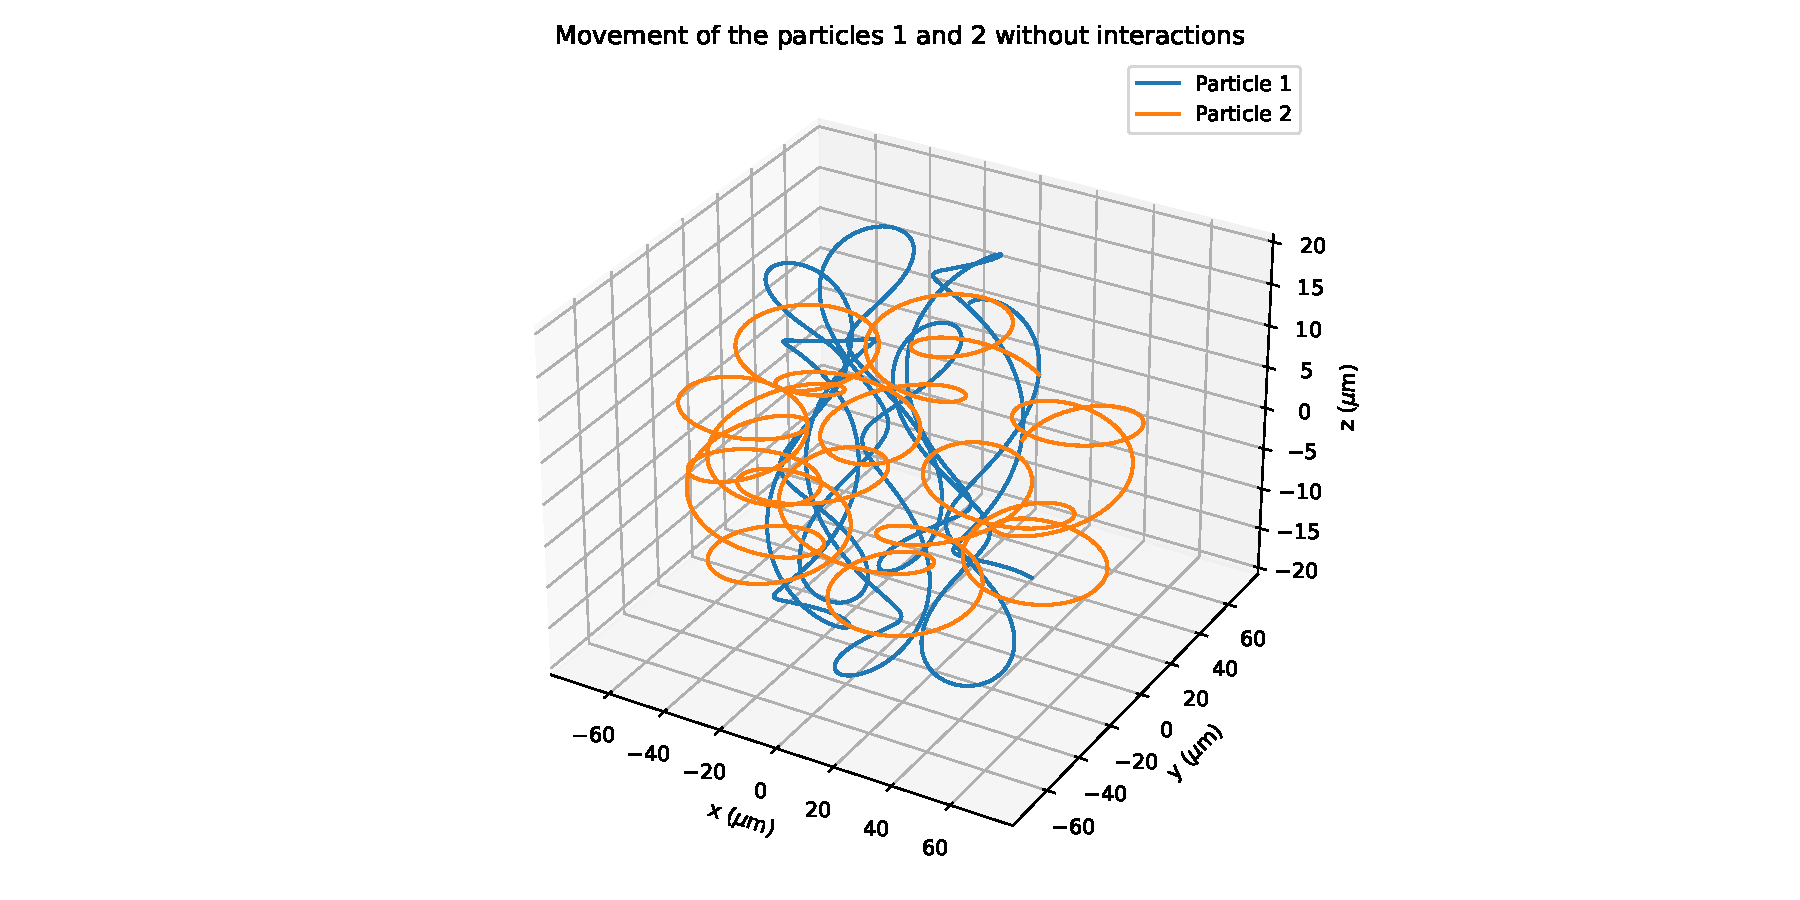
\includegraphics[width = .45\textwidth]{3Dwithoutinteractions.pdf} 
    \caption{3D plot showing the movement of particle 1 and particle 2 in the xyz-space without consideration to particle interaction. Saved as "3Dwithoutinteractions.pdf".}
    \label{fig: ee251}
\end{figure} 

\pagebreak
\subsubsection{Error analysis - relative error}
We want to make sure the model for the movement of particles within our penning trap is as accurate as possible, and to a degree that we deem satisfactory. To do so, we run multiple simulations for the movement of only particle 1 within our trap - this way we can use the theory for our special case of initial conditions. We write a code in c++ that estimates the movement of the particle by using both methods runge-kutta and forward-euler, for different steps n=4000, n=8000, n=16000, n=31000, and stores this data within .txt files that we import into python. Here, we use the formulas (13) and (17), in combination with the definitions of the special case of initial conditions of particle 1 presented in 2.3 to define the expected movement of the particle. Thereby, we estimate the relative error, as well as the error convergence rate using formulas (18), (19) and (20), and visualize the error in the case of both runge-kutta and forward-euler:
\begin{figure}[H]
    \centering
    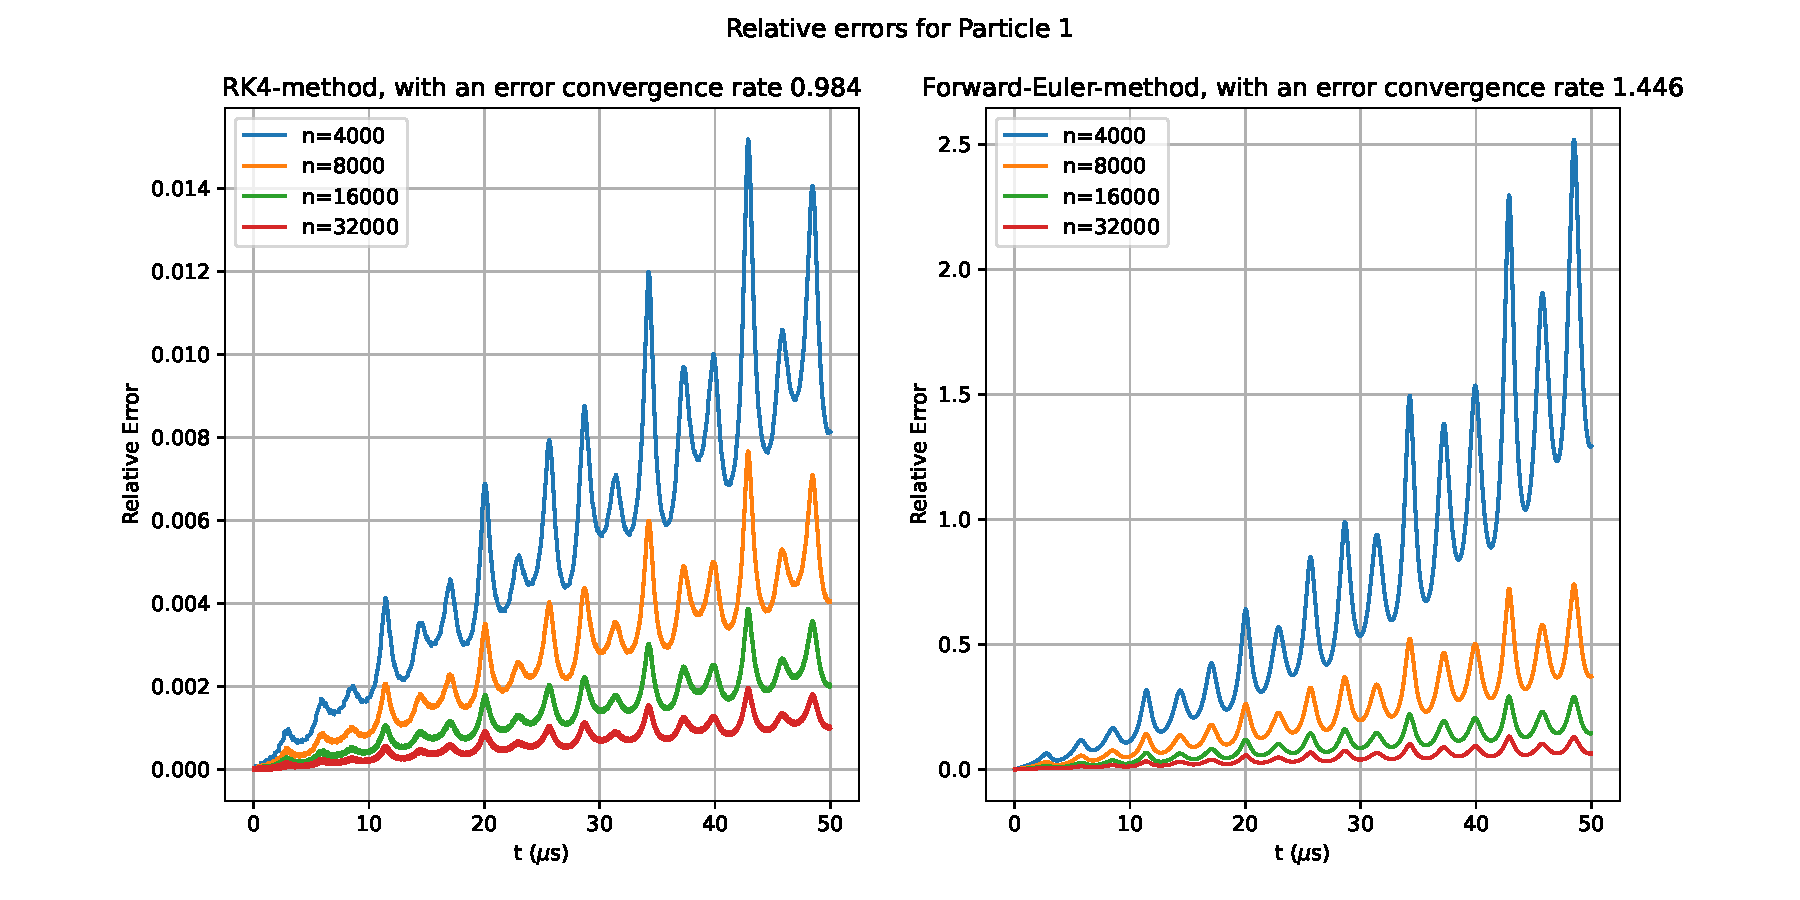
\includegraphics[width = .45\textwidth]{Relativeerror.pdf} 
    \caption{Figure visualizing the relative error at each time-step, for different amounts of time-steps, when movement of particle 1 within our system was calculated by both runge-kutta and forward-euler. The title of each subplot tells us the estimated convergence rate for both ODE-solvers. Saved as "Relativeerror.pdf".}
    \label{fig: ee251}
\end{figure} 
\begin{figure}[H]
    \centering
    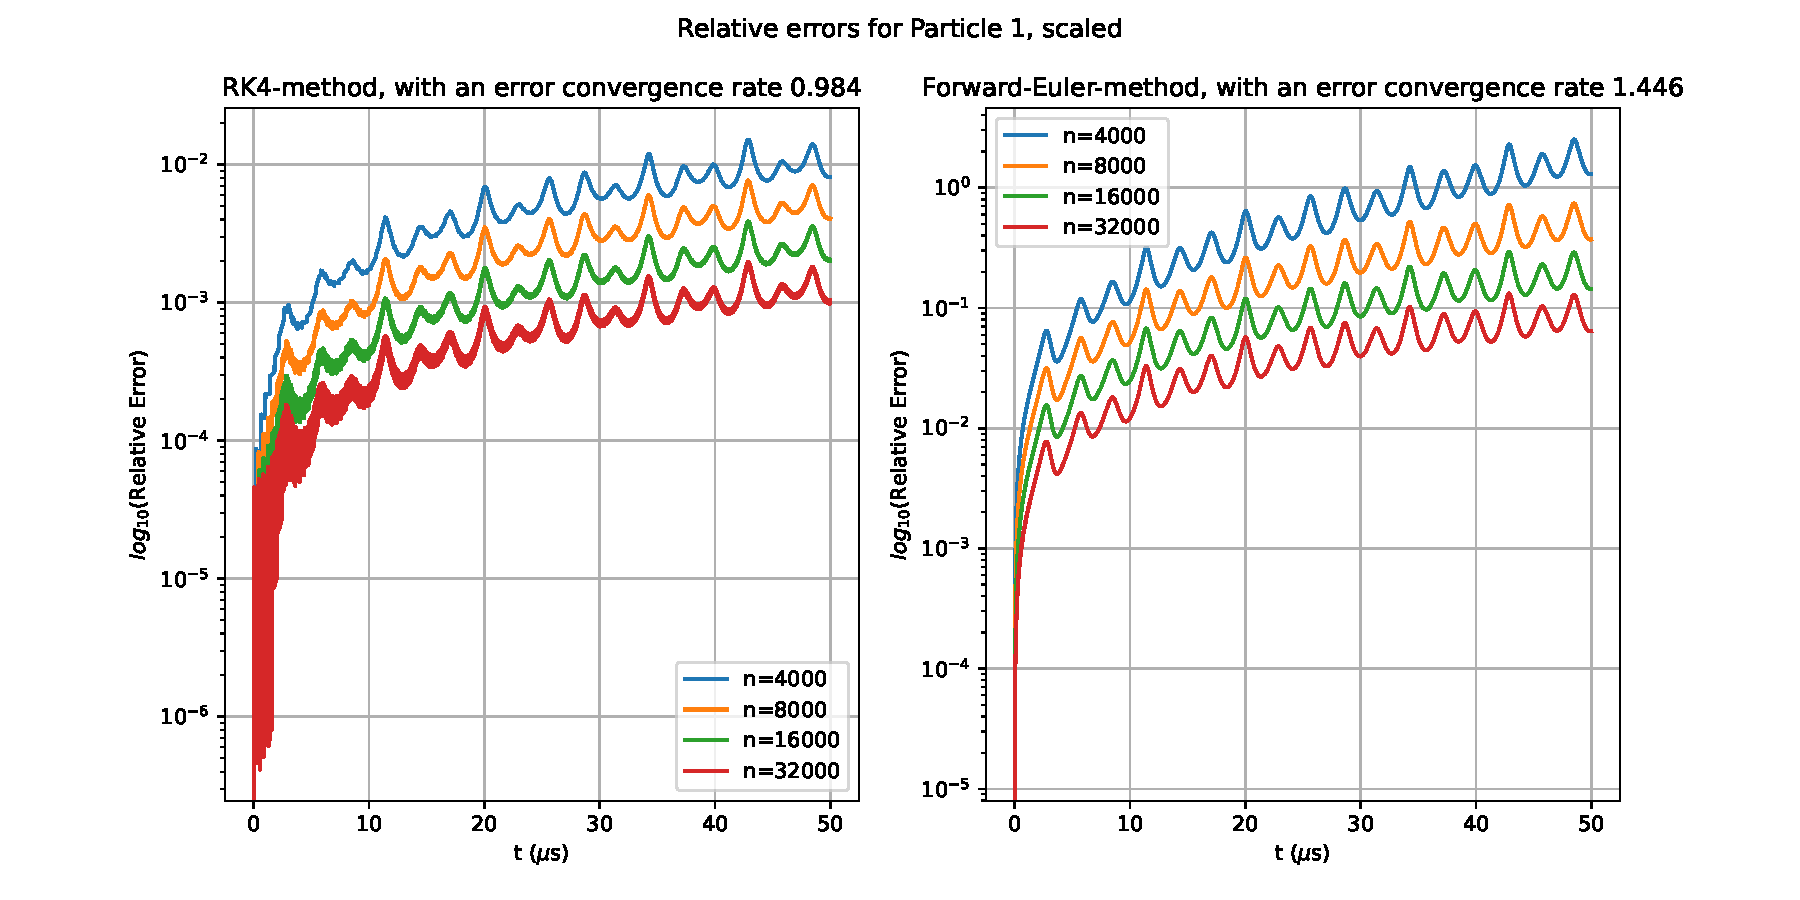
\includegraphics[width = .45\textwidth]{Relativeerrorformatted.pdf} 
    \caption{Figure showing the errors in Figure 10, formatted with a logarithmic scale in the y-axis. Saved as "Relativeerrorformatted.pdf".}
    \label{fig: ee251}
\end{figure} 

\subsubsection{Time dependency}
Up until now, we have only verified our model for the case of no time dependency, but the model has also been implemented to take into consideration time dependency in the electric-field potential. To test the model for time dependency, we make simulations for a trap-system containing 100 particles with randomly generated initial conditions for different amplitudes f=0.1,0.4,0.7, during a time interval $50 \mu s$ with 10000 time steps, and stores data on how many particles are still trapped within the system for each step in time, for each instance of amplitude f. This simulation is ran both with and without interaction between the particles, and then the data is imported into python where we visualize fraction of particles that are still trapped after the time interval as a function of $w_V$.
\begin{figure}[H]
    \centering
    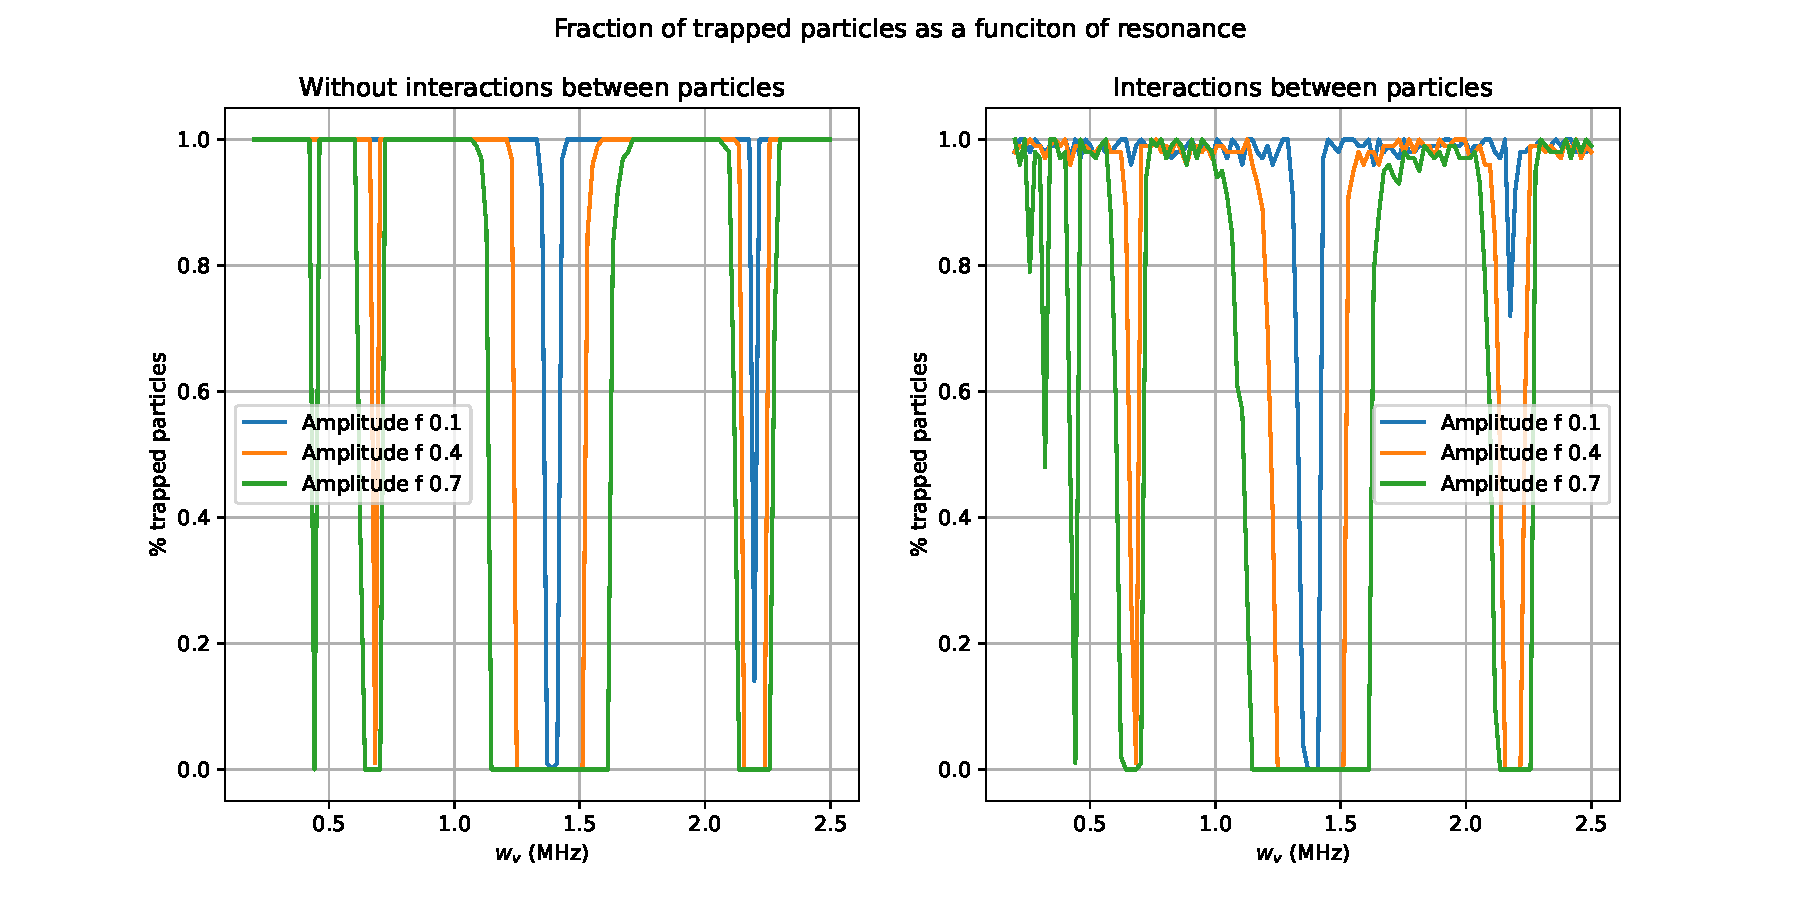
\includegraphics[width = .45\textwidth]{Trappedfrac.pdf} 
    \caption{Figure showing the fraction of trapped particles as a function of the angular frequency $w_V$, for different amplitudes f=0.1,0.4,0.7 with and without particle interactions. Saved as "Trappedfrac.pdf".}
    \label{fig: ee251}
\end{figure} 

By analyzing this plot presented in Figure 12, we can create another set of data and a new plot zooming into the interval of which the function for trapped particles resonances, $w_v \in [1.0 , 1.8]$.
\begin{figure}[H]
    \centering
    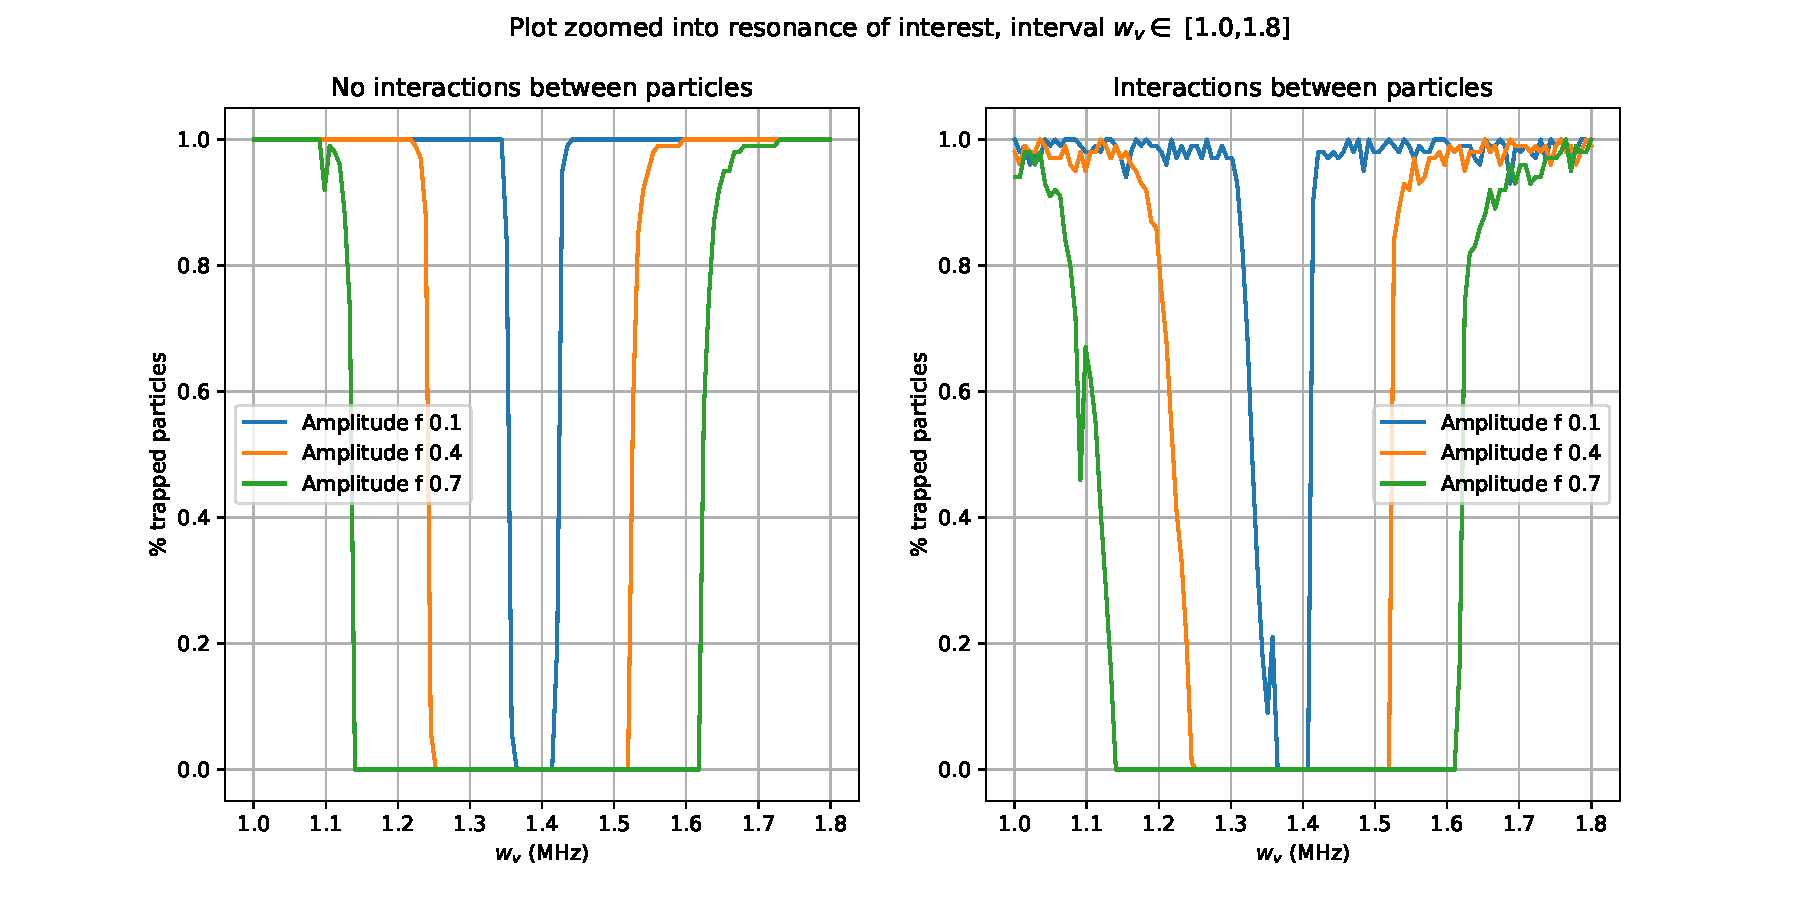
\includegraphics[width = .45\textwidth]{Trappedfraczoom.pdf} 
    \caption{Figure showing the fraction of trapped particles as a function of the angular frequency $w_v \in [1.0 , 1.8]$, for different amplitudes f=0.1,0.4,0.7 with and without particle interactions. Saved as "Trappedfraczoom.pdf".}
    \label{fig: ee251}
\end{figure} 




% ===========================================
\section{Discussion}\label{sec:discussion}
To check the accuracy of our implemented method runge-kutta, that we wish to make use of to estimate particle trajectories, we've ran the simulation for a single particle 1 within the penning trap, and compared the estimated movement with the expected movement in z-direction, visualized in Figure1. By running the simulation for different implementations of the runge-kutta method, and creating similar plots, I managed to create a trajectory-estimation method with as high degree of accuracy as possible. By rewriting the expression (13) for the expected trajectory of particle 1 \\
$z(t)=z_0\cos{w_zt} + \frac{v_{z0}}{w_z}sin(w_zt)$ with $v_{z0}=0:$ \\
$z(t)=z_0\cos{w_zt} + \frac{0}{w_z}sin(w_zt)$ with $z_0=20 \mu m$:\\
$z(t)=20\cos{w_zt}$ \\
it is clear that the plot does take the shape expected, given the value of $w_v$. \\

We check how our model handles particle interaction, by simulating both particles 1 and 2 in the same trap with and without interactions, and plot their trajectories in the xy-plane as visualized in Figure2. By further plotting this data in a dimension time as well, visualized in Figure3, we can clearly see how the two particles pull each other out of their path. The particle trajectories for the simulation taking interaction into consideration, looks as they've an extra rotation around each others path. This is as expected, due to Coulomb's law (9) between the particles. \\

Furthermore, we created plots showing the phase space (x,$v_x$) and (z,$v_z$) for the simulations of two particles, visualized in figures 4 and 6. These plots also got evolved in time to gain a better understanding of the physics in works, visualized in Figure 5 and 7. The phase space (z,$v_z$) transforms from a circular ratio, into one that seems to favor movement in the positive half of z-space. For the phase space in the x-dimension, we can see that the interaction between the particles keeps the particles trajectories in the negative half of the x-space. \\

We performed an error analysis for both runge-kutta and forward-euler methods for the trajectories of particle 1 in a penning trap, visualizing the relative error as a function of time, for increasing amount of time steps for our simulation, visualized in Figures 10 and 11. From these figures, we can read that in the case of both methods, an increasing amount of time steps results in a larger accuracy in trajectory estimations. The relative error is also way smaller in the case of runge-kutta method, which makes this method more reliable if we wish to create realistic simulations. The error convergence rate one can read from these plots Figure 10 and 11 further emphasises this assessment. \\

Finally, we wanted to test our model for time-dependency, which we did by simulating a system containing 100 particles within such a time-dependent model for the penning trap and monitoring how many particles escape the trap as a function of time. For both the case for and for no particle interaction, we plotted the fraction of particles within the trap as a function of $w_v$, visualized in both figures 12 and 13. The reason why we get resonance in our plot the way we do, is that there are certain frequencies $w_v$ that help more particles escape from our system. This can be deduced from the formula for time-dependent electric field (8), and that when this expression is at its max - which is dependent on $w_v$, the force from the electric field will be at a max, and subsequently help more particles escape from the trap. One would expect a peak in the field strength, whenever $cos(w_vt)$ is at a max, which would happen whenever $w_vt=0,\pi, 2\pi, ...$, which is a pattern we observe in our figures. Furthermore, expression (8) tells us that the strength of the electric field will increase with an increasing amplitude f, which we can confirm by looking at Figure 12. \\

By examining our zoomed-in plot, Figure 13, one can draw the conclusion that the structure of resonances do not seem to be greatly affected by, if affected at all, the simulation's consideration to particle interaction. This may be because the forces between the particles have sizes or a net direction that does not affect particles' ability to escape the penning trap in a large enough degree. The effect the electric field has on the particles is large compared to the effect the particles have on each other. \\


% ===========================================
\section{Conclusion}\label{sec:conclusion}
In this project, we examined data collected by utilizing a model created for a penning trap. By visualizing and comparing simulation data to our expectations, we discussed the accuracy of the model and how to use it to obtain accurate simulation results. We can conclude that our model for a penning trap, accounting for particle interactions and time-dependent factors, has a high degree of accuracy. For researchers aiming to achieve the most precise estimations of particle trajectories, we recommend the utilization of the Runge-Kutta method.

After affirming the accuracy of our model, we took a closer look at the physics at works within our system.
We confirm that the penning trap is indeed a powerful tool for manipulation of particle trajectories, and consequently also a good tool for particle confinement.
\section{References}\label{sec:references}


\bibliography{ref}
\textbf{Project 3 assignment text}

\end{document}